\documentclass[a4paper]{article}
\usepackage{amsmath}
\usepackage{amssymb}
\usepackage{braket}%量子力学符号
\usepackage{geometry}
\usepackage{enumerate}
\usepackage{natbib}
\usepackage{float}%稳定图片位置
\usepackage{graphicx,subfig}%画图
\usepackage{caption}
\usepackage[english]{babel}
\usepackage{indentfirst}%缩进
\usepackage{enumerate}%加序号
\usepackage{multirow}%合并行
\usepackage{hyperref}
\hypersetup{hypertex=true, colorlinks=true, linkcolor=black, anchorcolor=black, citecolor=black}
\title{\Large \textbf{VP390 Problem Set 5}\\
\author{\textbf{Pan, Chongdan ID:516370910121}\\
}
}
\begin{document}
\maketitle
\section{Problem 1}
\begin{enumerate}[(b)]
    \item Assume $\psi$ is the solution for $-\frac{\hbar^2}{2m}\frac{\mathrm{d}^2\psi(x)}{\mathrm{d}x^2}+V(x)\psi(x)=E\psi(x)$
    \\Then $-\frac{\hbar^2}{2m}\frac{\mathrm{d}^2\psi(-x)}{\mathrm{d}x^2}+V(-x)\psi(-x)=E\psi(-x)$
    \\Since $V(x)=V(-x)$
    \\$-\frac{\hbar^2}{2m}\frac{\mathrm{d}^2\psi(-x)}{\mathrm{d}x^2}+V(x)\psi(-x)=E\psi(-x)$
    \\$\psi(-x)$ also satisfies this stationery equation.
    \\Therefore $\psi(x)\pm\psi(-x)$ satisfies this equation as well. 
\end{enumerate}
\section{Problem 2}
\begin{enumerate}[(a)]
    \item When $x<0,\Psi(x)=0$
    \\When $x>a,\Psi(x)=Ae^{-\kappa_1x}$, where $\kappa_1^2=-\frac{2mE}{\hbar^2}$
    \\When $0\leq x\leq a,V(x)=-V_0\rightarrow\frac{\partial^2\Psi(x)}{\partial x^2}+\frac{2m}{\hbar^2}(E+V_0)\Psi(x)=0$
    \\Let $\kappa_2=\sqrt{\frac{2m}{\hbar^2}(E+V_0)},\Psi(x)=C_1\cos\kappa_2x+C_2\sin\kappa_2x$
    \\$\Psi(0)=0\rightarrow C_1=0$
    \\$\Psi(a)'=-A\kappa_1e^{-\kappa_1a}=\kappa_2C_2\cos\kappa_2a\rightarrow C_2=\frac{A\kappa_1e^{-\kappa_1a}}{\kappa_2\cos\kappa_2a}$
    \\$\int_{-\infty}^\infty||\Psi(x)||^2\mathrm{d}x=\int_0^a(\frac{A\kappa_1e^{-\kappa_1a}}{\kappa_2\cos\kappa_2a}\cos\kappa_2x)^2\mathrm{d}x+\int_a^\infty A^2e^{-2\kappa_1x}\mathrm{d}x=1$
    \\$\frac{A^2}{2\kappa_1}e^{-2\kappa_1x}+(\frac{A\kappa_1e^{-\kappa_1a}}{\kappa_2\cos\kappa_2a})^2\frac{\sin(2a\kappa_2)+2a\kappa}{4\kappa_2}=1$
    \\$A=\sqrt{\frac{8\kappa_1\kappa_2(\kappa_2\cos\kappa_2a)^2}{e^{-2\kappa_1x}4\kappa_2(\kappa_2\cos\kappa_2a)^2+2\kappa_1(\sin(2a\kappa_2)+2a\kappa)(\kappa_1e^{-\kappa_1a})^2}}$
    \\$\kappa_1^2+\kappa_2^2=\frac{2m}{\hbar^2}V_0$
    \\Since the bound states only exists when $x>0$, which has the similar form with finite well when $\psi$ is odd, then the bound states are only the original odd wave bound states in finite well problem.
    \item The solution when $x>a$ has the same form of solution with same value of $\kappa_1,\kappa_2$, only $C_2,A$ need recalculated. For $0\leq x\leq a$, it has the same form as the odd solution with finite potential well.
    \\When $x<-a,\Psi(x)=Be^{-\kappa_1x}$, where $\kappa_1^2=-\frac{2mE}{\hbar^2}$
    \\When $x>a,\Psi(x)=Ae^{-\kappa_1x}$
    \\When $0\leq x\leq a$, If the $\psi$ is odd, $\psi=C\sin\kappa_2x$, which has the solution of same form with this problem's.
    \item According to Figure.\ref{odd} shows that only first bound state is for even function.
    \begin{figure}[H]
        \centering
        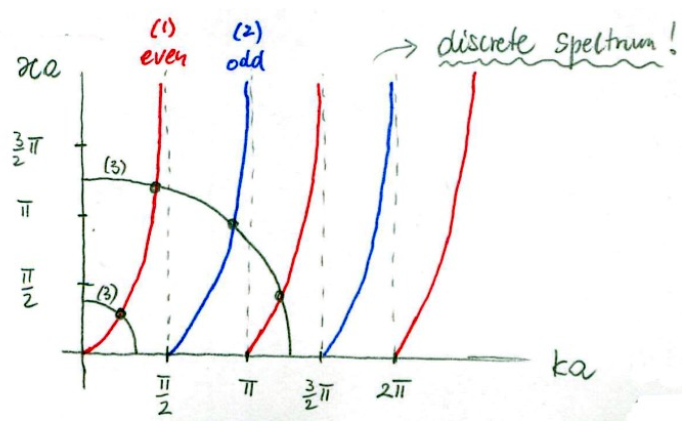
\includegraphics[scale=0.3]{P1.png}
        \caption{Energy level for finite well}
        \label{odd}
    \end{figure}
    Therefore, it's possible to set the width and the depth of the well so that there is no bound state or only one bound state.
    \item According to above graph, to have only one bound states in odd function, the radius should $\frac{\pi}{2}\leq r<\frac{3\pi}
    {2})$
    \\Since $a=r\sqrt{\frac{\hbar^2}{2mV_0}}$
    \\Then $1.62\times10^{-10}m\leq r<4.85\times10^{-10}m$
\end{enumerate}
\section{Problem 3}
\noindent$-\frac{\hbar^2}{2m}\frac{\partial^2\Psi(x)}{\partial x^2}-E\Psi(x)=V_0\delta(x)\Psi(x)$
\\Integrate the equation over an infinitesimal interval $[-\varepsilon,\varepsilon]$, we get:
\\$$-\frac{\hbar^2}{2m}(\Psi(\varepsilon)'-\Psi(-\varepsilon)')-E\int_{-\varepsilon}^\varepsilon\Psi(x)\mathrm{d}x=V_0\Psi(0)$$
\\When $x\neq0,\frac{\partial^2\Psi(x)}{\partial x^2}+\frac{2m}{\hbar^2}E\Psi(x)=0$
\\When $x<0,\Psi(x)=Ae^{\kappa x}$, where $\kappa^2=-\frac{2mE}{\hbar^2}$
\\When $x>0,\Psi(x)=Be^{-\kappa x}$
\\Since $\Psi(x)$ should be continuous, $\Psi(0)=A=B$, hence $\Psi(x)$ is even because $V(x)$ is symmetric.
\\Then $\Psi(\varepsilon)'=-\Psi(-\varepsilon)'$, and the original integral equation becomes: 
\\$$\Psi(\varepsilon)'=-\frac{m}{\hbar^2}(E\int_{-\varepsilon}^\varepsilon\Psi(x)\mathrm{d}x+V_0\Psi(0))=\frac{m}{\hbar^2}[2E\frac{A}{\kappa}(e^{-\kappa\varepsilon}-1)-V_0\Psi(0)]$$
\\$\lim_{\varepsilon\rightarrow0}\Psi(\varepsilon)'=-\frac{m}{\hbar^2}V_0A\neq 0$, hence $\Psi(x)'$ is not continuous at $x=0$
\\For normalization $\int_{-\infty}^0|Ae^{\kappa x}|^2\mathrm{d}x+\int_0^{\infty}|Ae^{-\kappa x}|^2\mathrm{d}x=1$
\\$\frac{A^2}{\kappa}=1\rightarrow A=\sqrt{\kappa}$
\\Plug it back, when $x>0$, we get $\Psi(x)'=\kappa^\frac{3}{2}e^{-\kappa x}=\frac{mA}{\hbar^2}[2E\frac{1}{\kappa}(e^{-\kappa x}-1)-V_0]$
\\Then we get $-\frac{2E}{\kappa}=V_0\rightarrow E=-\frac{V_0^2m}{2\hbar^2}$
\section{Problem 4}
    \begin{enumerate}
        \item $\Psi(x,0)=\sqrt{\frac{1}{3}}\psi_3+\sqrt{\frac{2}{3}}\psi_5$
        \\where $\psi_n=C_nH_n(\frac{x}{x_0})e^{-\frac{1}{2}(\frac{x}{x_0})^2},C_n=\frac{1}{\sqrt{2^nn!x_0\sqrt{\pi}}},x_0=\sqrt{\frac{\hbar}{m\omega}}$
        \\$\braket{\Psi_n,\Psi_m}=\int_{-\infty}^\infty\Psi_n^*\Psi_m\mathrm{d}x=\int_{-\infty}^\infty H_n(\frac{x}{x_0})H_m(\frac{x}{x_0})C_nC_me^{-(\frac{x}{x_0})^2}\mathrm{d}x$
        \\Let $y=\frac{x}{x_0},$ then $\braket{\Psi_n,\Psi_m}=\int_{-\infty}^\infty H_n(y)H_m(y)C_nC_me^{-y^2}x_0\mathrm{d}y$
        \\According to the property, when $m\neq n$, $\int_{-\infty}^\infty H_n(y)H_m(y)F(y)\mathrm{d}y=0$
        \\Thus $\braket{\Psi_n,\Psi_m}=0$, and the eigenfunction is orthogonal.
        \\When $n=m,\braket{\Psi_n,\Psi_m}=\int_{-\infty}^\infty H_n(y)^2C_n^2e^{-y^2}x_0\mathrm{d}y=\frac{x_0}{2^nn!x_0\sqrt{\pi}}\int_{-\infty}^\infty H_n(y)^2e^{-y^2}\mathrm{d}y$
        \\Since $\int_{-\infty}^\infty H_n(y)^2e^{-y^2}\mathrm{d}y=2^nn!\sqrt{\pi}\delta_{nn}=2^nn!\sqrt{\pi}$
        \\Then $\braket{\Psi_n,\Psi_n}=C_n^22^nn!\sqrt{\pi}=1$, so each eigenfunction is normalized.
        \\\\$\braket{\Psi,\Psi}=\braket{\sqrt{\frac{1}{3}}\psi_3,\sqrt{\frac{1}{3}}\psi_3}+\braket{\sqrt{\frac{1}{3}}\psi_3,\sqrt{\frac{2}{3}}\psi_5}+\braket{\sqrt{\frac{2}{3}}\psi_5,\sqrt{\frac{1}{3}}\psi_3},\braket{\sqrt{\frac{2}{3}}\psi_5+\sqrt{\frac{2}{3}}\psi_5}$
        \\$=\frac{1}{3}\braket{\psi_3,\psi_3}+0+0+\frac{2}{3}\braket{\psi_5,\psi_5}=\frac{1}{3}+\frac{2}{3}=1$
        \\So it's normalized
        \item $\Psi(x,0)=\sqrt{\frac{1}{144x_0\sqrt{\pi}}}[8(\frac{x}{x_0})^3-12\frac{x}{x_0}]e^{-\frac{1}{2}(\frac{x}{x_0})^2}+\sqrt{\frac{1}{5760x_0\sqrt{\pi}}}[32(\frac{x}{x_0})^5-160(\frac{x}{x_0})^3+120\frac{x}{x_0}]e^{-\frac{1}{2}(\frac{x}{x_0})^2}$
        \\where $x_0=\sqrt{\frac{\hbar}{m\omega}}$
        \item The possible outcome of energy is $E_3=\frac{7}{2}\hbar\omega,E_5=\frac{11}{2}\hbar\omega$
        \\The probability to get $E_3$ is $\frac{1}{3}$, for $E_5$ is $\frac{2}{3}$
        \item $E=\frac{1}{3}E_3+\frac{2}{3}E_5=\frac{29}{6}\hbar\omega$
        \item $\Psi(x,t)=\sqrt{\frac{1}{3}}e^{\frac{i}{\hbar}E_3t}\psi_3(x)+\sqrt{\frac{2}{3}}e^{\frac{i}{\hbar}E_5t}\psi_5(x)$
    \end{enumerate}
\section{Problem 5}
    \begin{enumerate}[(a)]
        \item Let $y=\frac{x}{x_0}$
        \\When $n=m,\braket{\Psi_n,\Psi_m}=\int_{-\infty}^\infty H_n(y)^2C_n^2e^{-y^2}x_0\mathrm{d}y=\frac{x_0}{2^nn!x_0\sqrt{\pi}}\int_{-\infty}^\infty H_n(y)^2e^{-y^2}\mathrm{d}y$
        \\Since $\int_{-\infty}^\infty H_n(y)^2e^{-y^2}\mathrm{d}y=2^nn!\sqrt{\pi}\delta_{nn}=2^nn!\sqrt{\pi}$
        \\Then $\braket{\Psi_n,\Psi_n}=C_n^22^nn!\sqrt{\pi}=1$, so each eigenfunction is normalized.
        \item According to text book: $\int_{-\infty}^\infty\psi_n^*x\psi_m\mathrm{d}x=0$ unless $n=m\pm1$
        \\Then $\braket{x}=\int_{-\infty}^\infty\psi_n^*x\psi_n\mathrm{d}x=0$, and $\braket{p}=0$
        \\Therefore $\bigtriangleup x=\sqrt{\braket{x^2}}=C_1^2\int_{-\infty}^\infty H_1(\frac{x}{x_0})^2x^2e^{-(\frac{x}{x_0})^2}\mathrm{d}x$
        \\$\bigtriangleup p=\sqrt{\braket{p^2}}=C_1^2\int_{-\infty}^\infty -\hbar H_1(\frac{x}{x_0})e^{-\frac{1}{2}(\frac{x}{x_0})^2}\frac{\partial^2H_1(\frac{x}{x_0})e^{-\frac{1}{2}(\frac{x}{x_0})^2}}{\partial x^2}\mathrm{d}x$
        \\Then for the ground state $\bigtriangleup x\bigtriangleup p=\frac{\hbar}{2}$
        \begin{figure}[H]
            \centering
            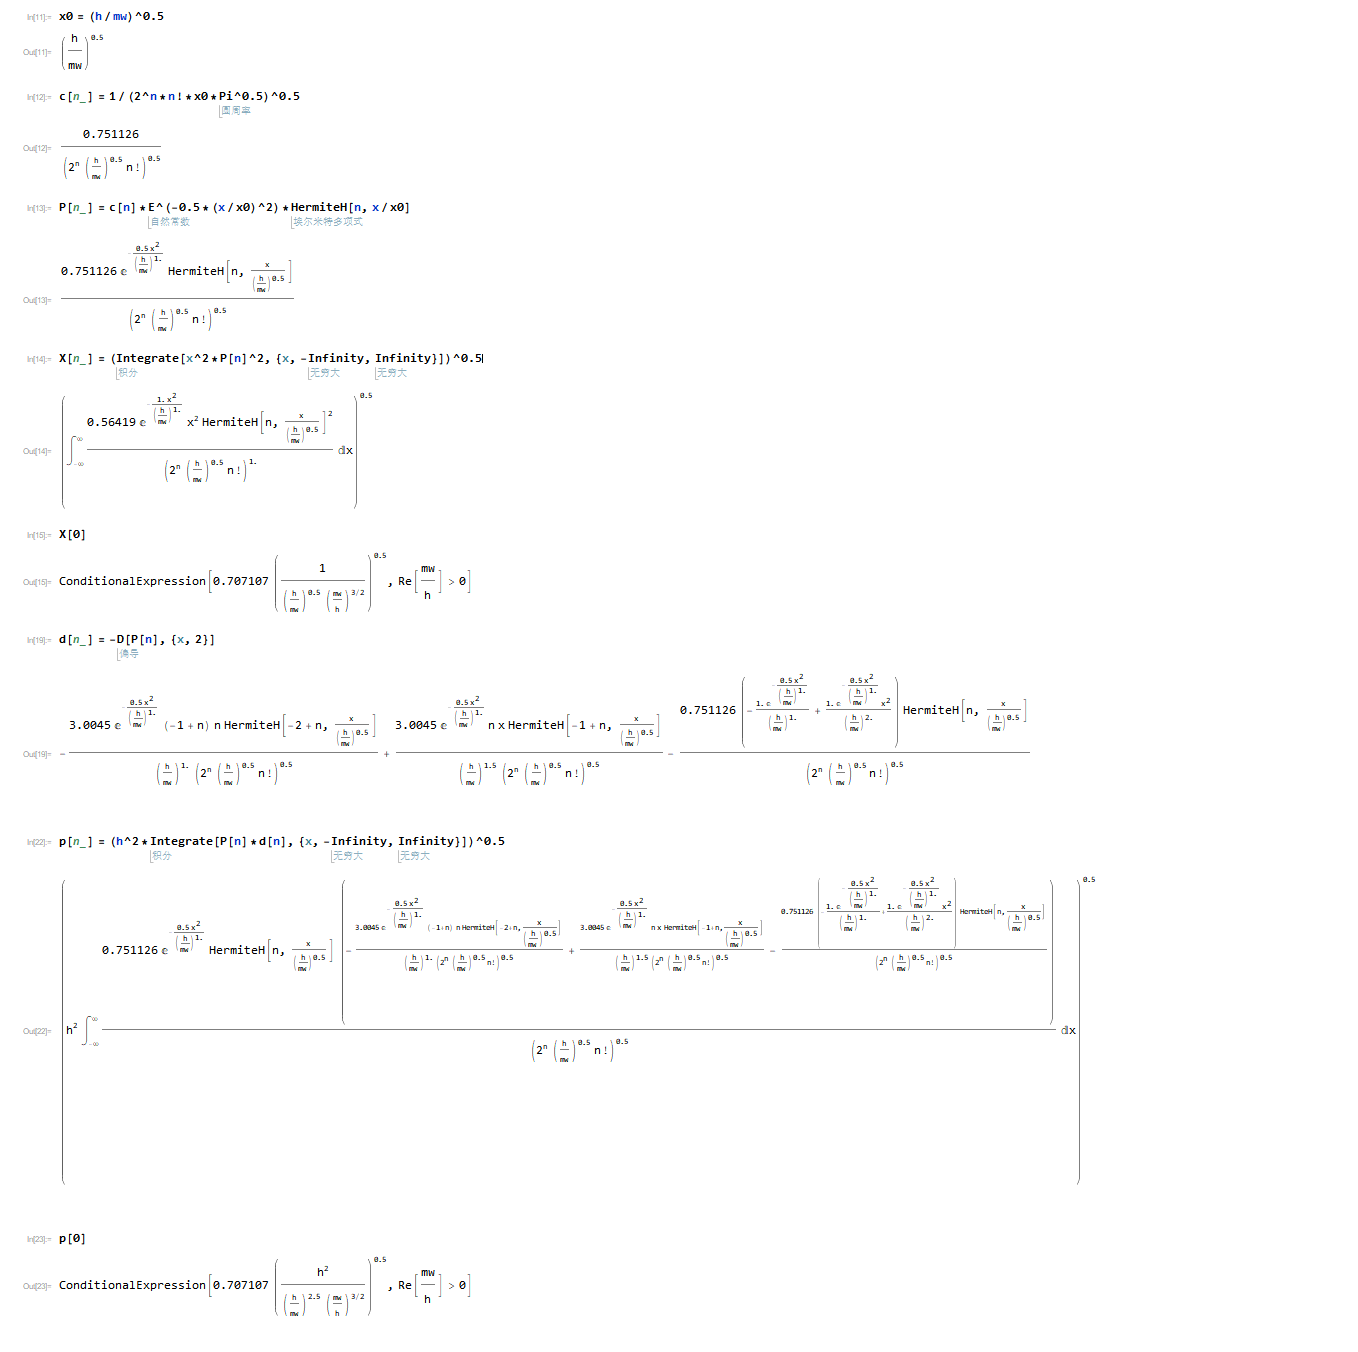
\includegraphics[scale=0.25]{P2.png}
            \caption{Mathematica Code for Integral Calculation}
            \label{Code}
        \end{figure}
        According to the Mathematica code in Figure.\ref{Code} and test result for larger $n$, we know that $\bigtriangleup x=\sqrt{\frac{\hbar}{2m\omega}},\bigtriangleup p=\sqrt{\frac{m\omega\hbar}{2}}$ and $\bigtriangleup x\bigtriangleup p=\frac{\hbar}{2}$ for ground state.
        \begin{figure}[H]
            \centering
            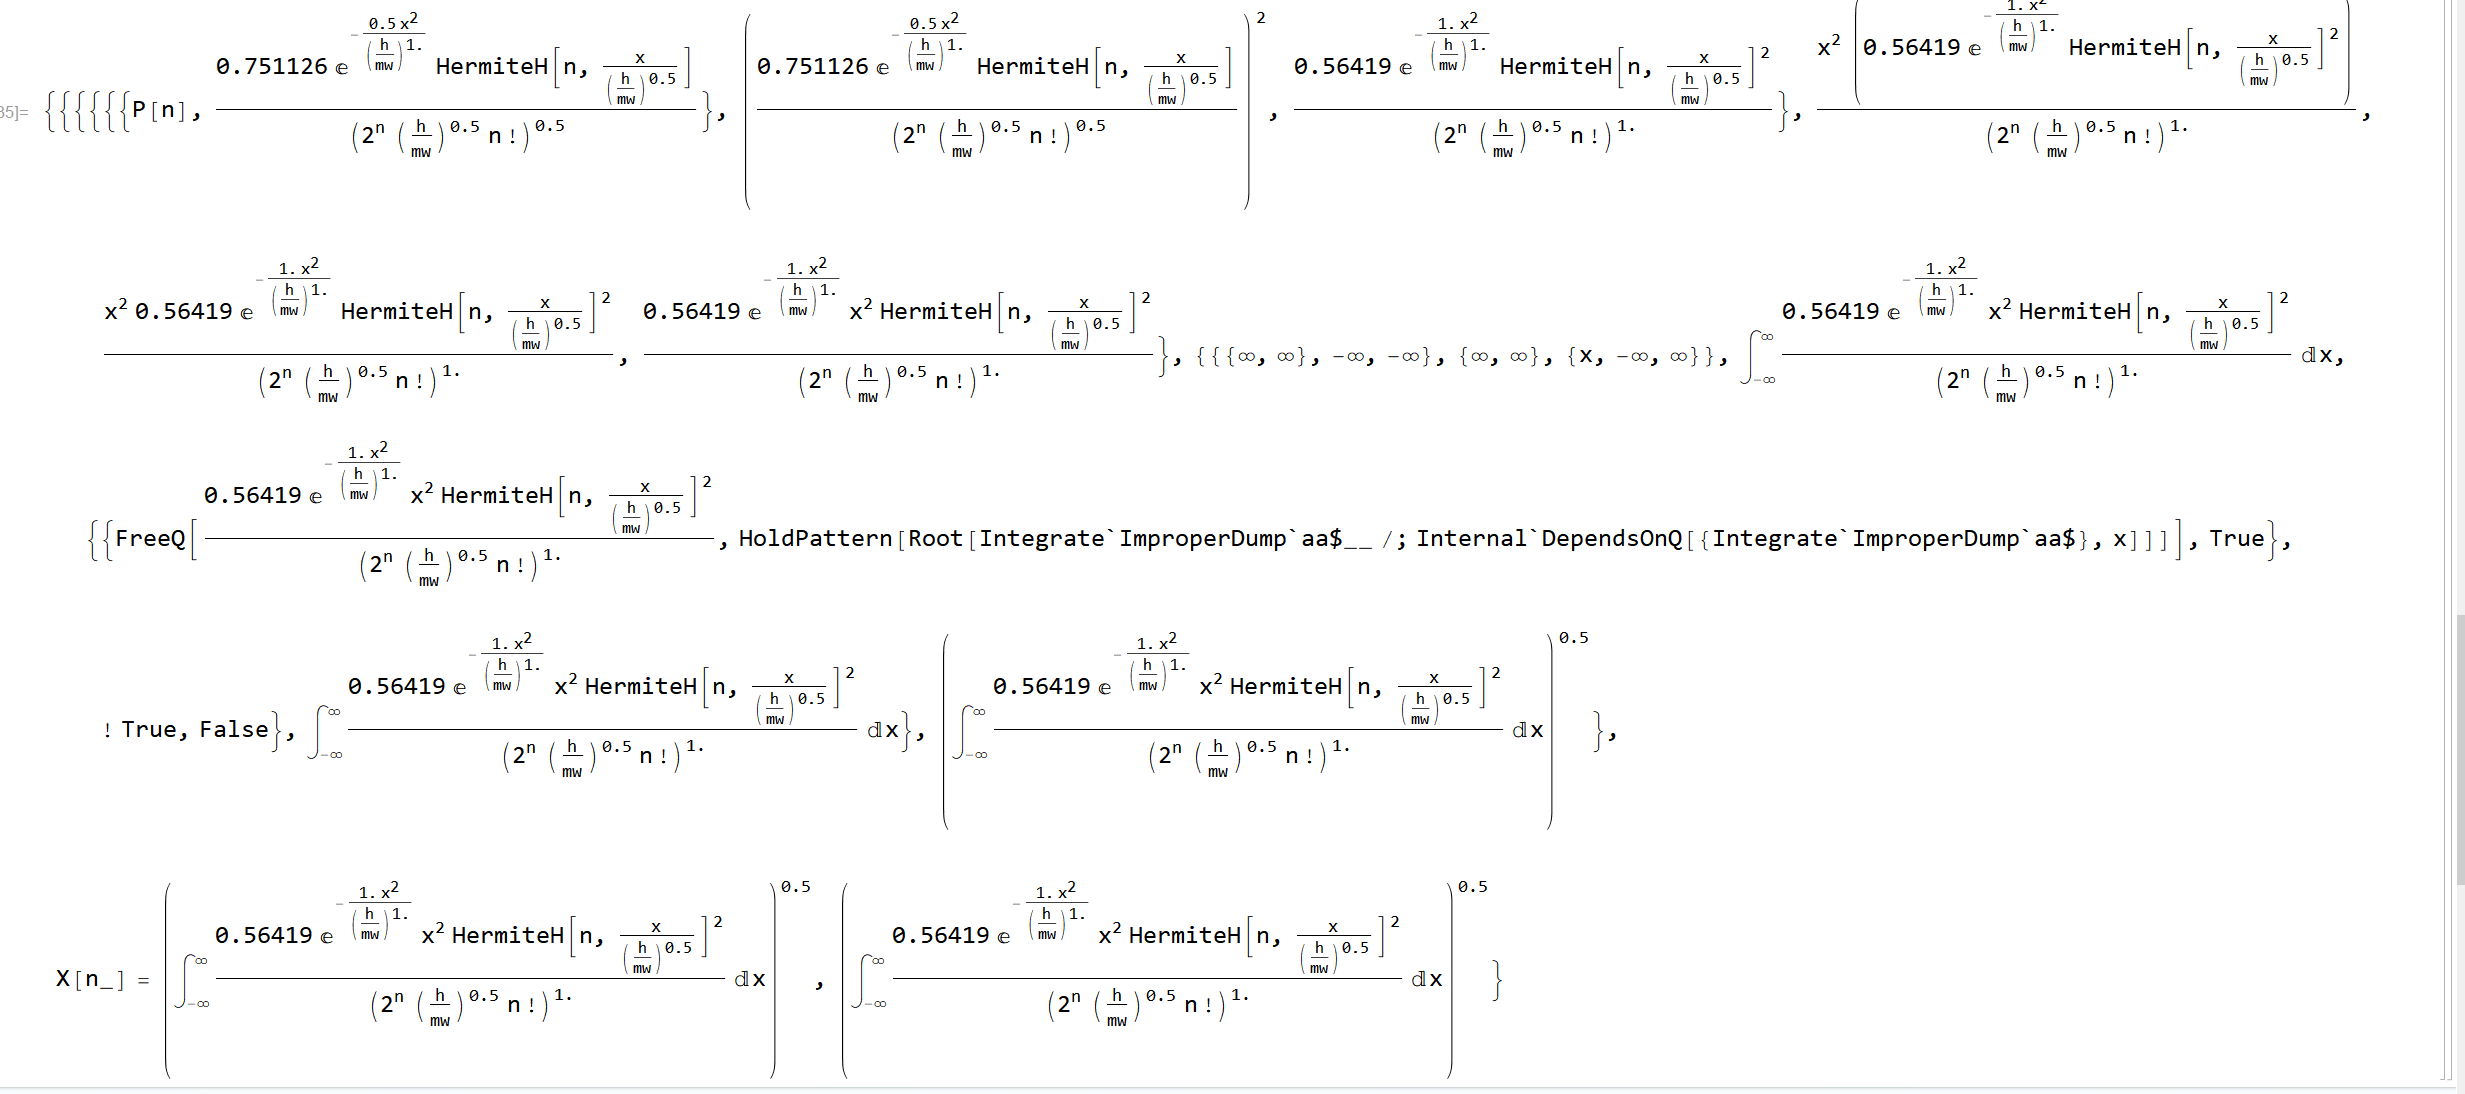
\includegraphics[scale=0.2]{P3.png}
            \caption{Calculation procedure for Mathematica to find $\bigtriangleup x$}
            \label{x}
        \end{figure}
        \begin{figure}[H]
            \centering
            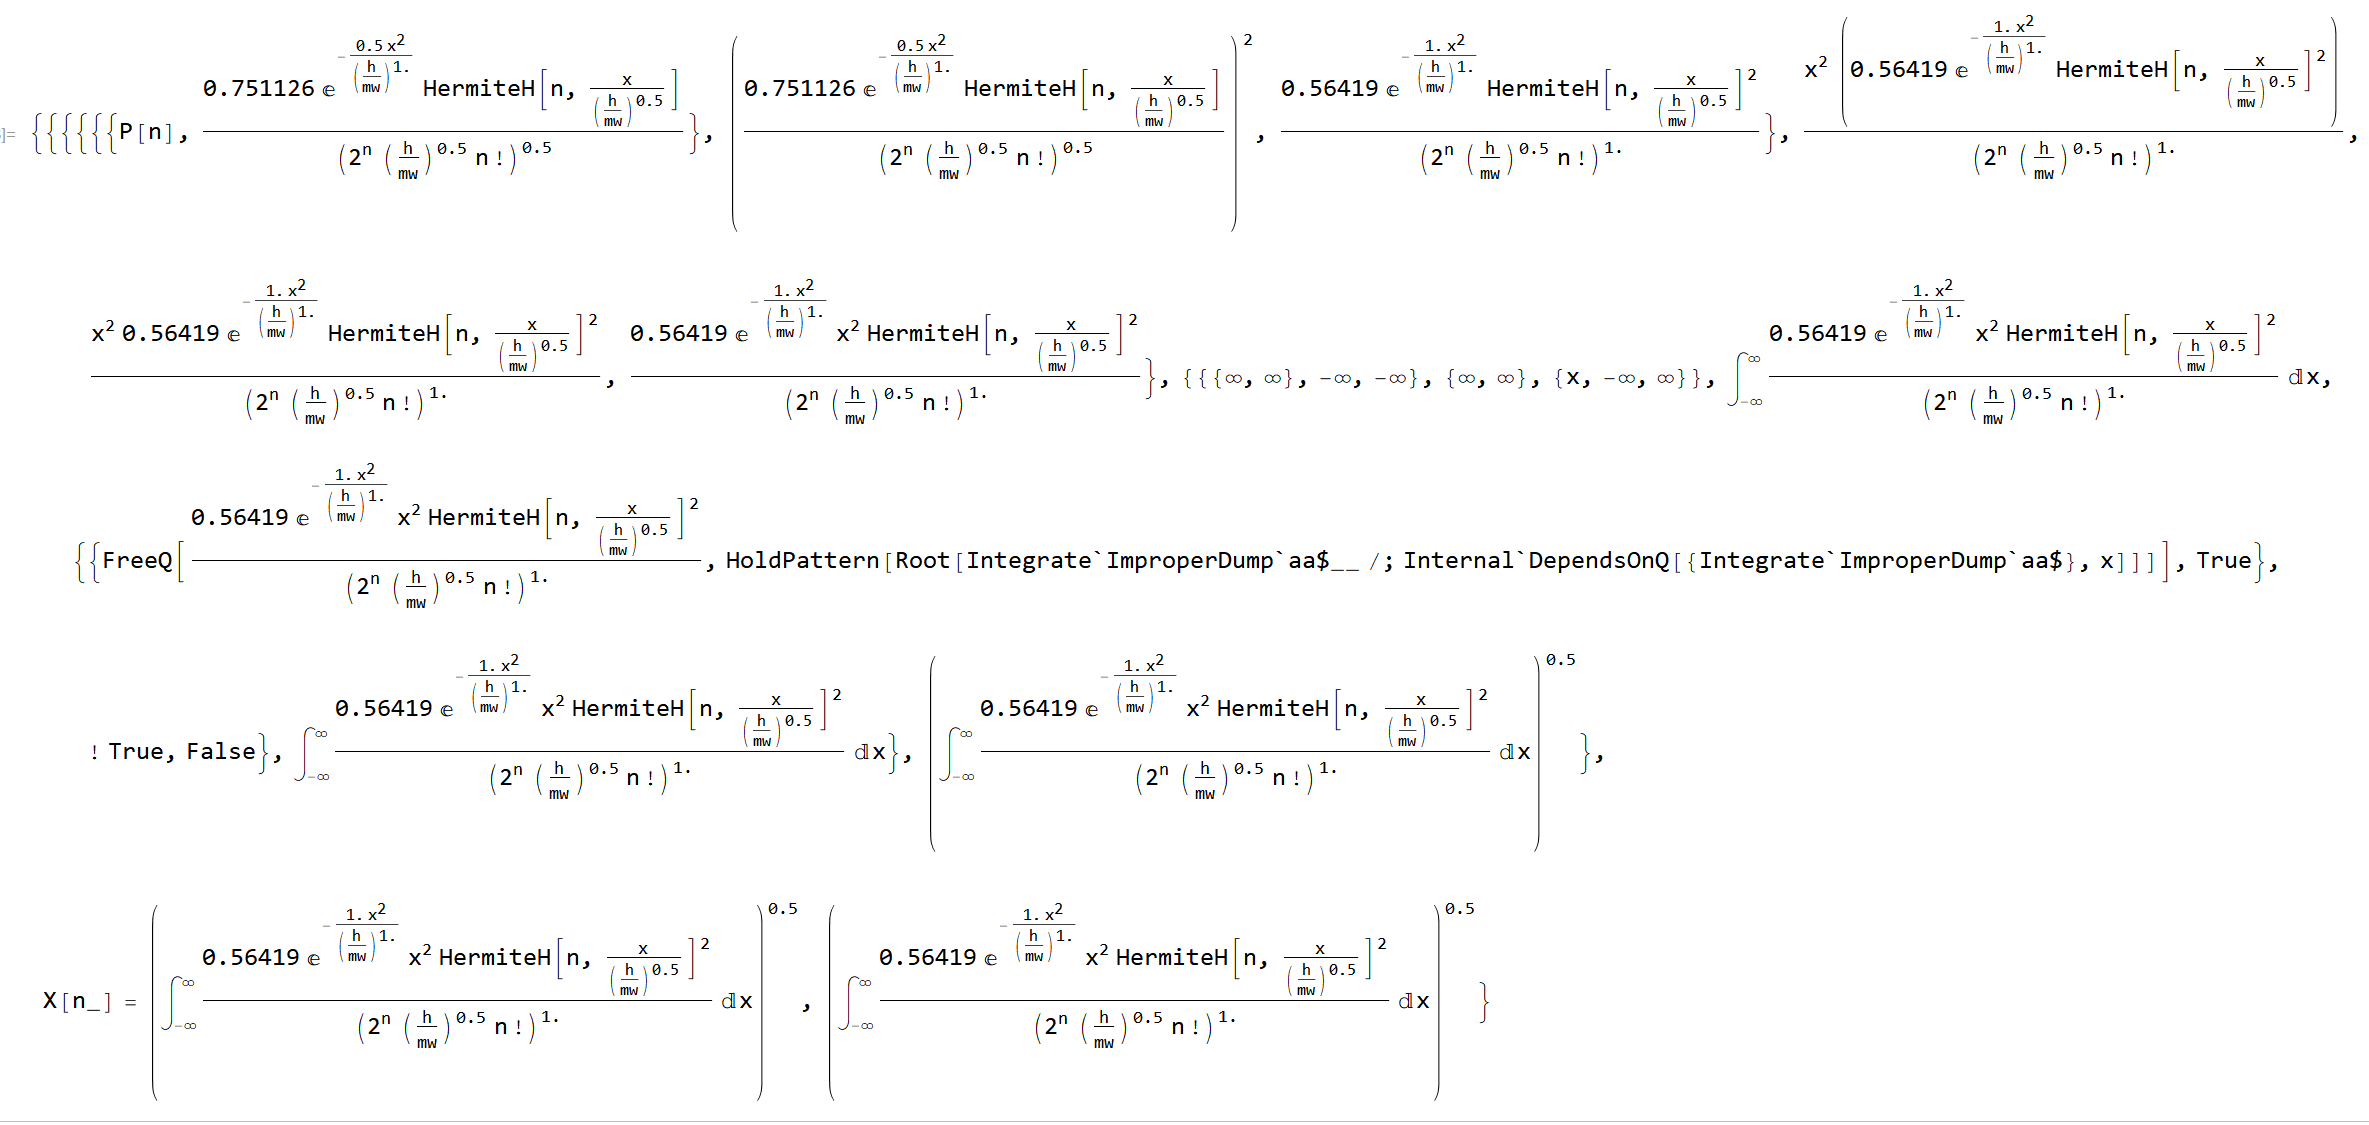
\includegraphics[scale=0.2]{P4.png}
            \caption{Calculation procedure for Mathematica to find $\bigtriangleup p$}
            \label{p}
        \end{figure}
        According to Figure.\ref{x} and Figure.\ref{p}, we know that the value of $\bigtriangleup x$ and $\bigtriangleup p$ increase with $n$, hence their product increases with n, and $\bigtriangleup x\bigtriangleup p\geq\frac{\hbar}{2}$
        \item $\hat{K}=-\frac{\hbar^2}{2m}\frac{\partial^2}{\partial x^2}$, hence $\bar{K}=\frac{(\bigtriangleup p)^2}{2m}$
        \\$\hat{V}=V(x)=\frac{1}{2}m\omega^2x^2$, hence $\bar{V}=\frac{m\omega^2}{2}(\bigtriangleup x)^2$
        \\Therefore $\bar{K}\bar{V}=\frac{\omega^2}{4}(\bigtriangleup x\bigtriangleup p)^2\geq\frac{\hbar\omega^2}{16}$
        \\When it's ground state, we plug the value of $\bigtriangleup_x,\bigtriangleup_p$:
        \\We get $\bar{K}=\frac{\omega\hbar}{4},\bar{V}=\frac{\omega\hbar}{4}$, then $\bar{K}=\bar{V}=\frac{E_0}{2}$
        \begin{figure}[H]
            \centering
            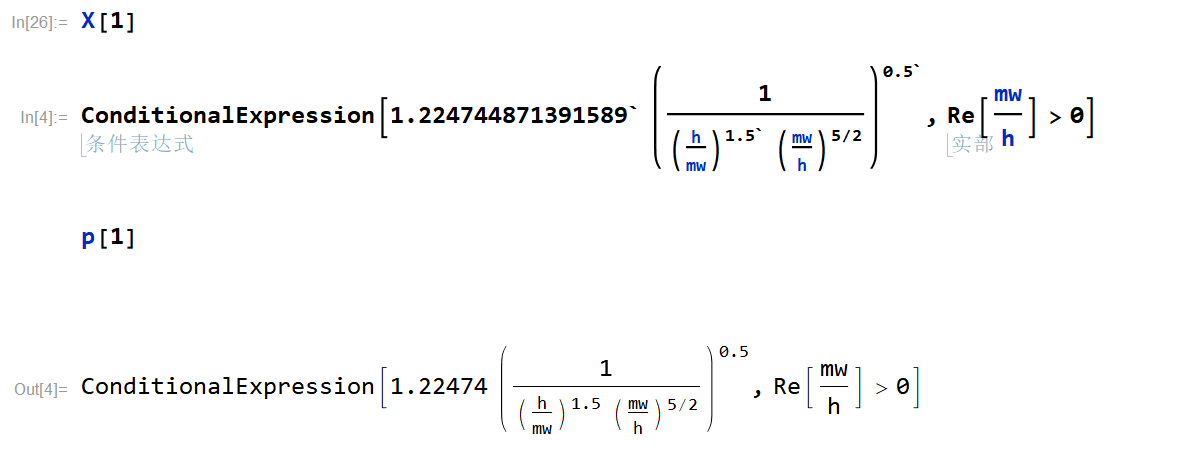
\includegraphics[scale=0.25]{P5.png}
            \caption{The coefficients are same}
            \label{Coefficient}
        \end{figure}
        According to Mathematica result in Figure.\ref{Coefficient} in question (b), we can find that the coefficients before $\bigtriangleup_x,\bigtriangleup_p$ are same.
        \\Therefore, for all n-eigenstates, $\bar{K}=\bar{V}=\frac{E_0}{2}$
    \end{enumerate}
\section{Problem 6}
\begin{enumerate}[(a)]
    \item Assume the center of the cube as the original point. If the electron displacement is $x$, then we can imagine it's in a ball with radius $x$, with bound charge $Q'=\frac{Q}{L^3}\frac{4\pi x^3}{3}$, since the electric field caused by outside potential and chare is symmetric, we only need to calculate the electric field caused by internal charge for the oscillation model. According to Gauss Law: 
    \\$4\pi x^2E=\frac{Q'}{\epsilon_0}\rightarrow E=\frac{Qx}{3\epsilon_0L^3}$
    \\Then the spring constant $A=\frac{qE}{x}=\frac{Qe}{3\epsilon_0L^3}$
    \item The original harmonic oscillator equation is $-\frac{\hbar^2}{2m}\frac{\partial^2\psi(x)}{\partial x^2}+\frac{m\omega^2x^2}{2}\psi(x)=E\psi(x)$, where $V(x)=\frac{1}{2}m\omega^2x^2$ 
    \\In our equation $V(x)=\frac{1}{2}m\omega^2x^2+\frac{e\Phi_0}{L}x=\frac{1}{2}m\omega^2(x+\frac{e\Phi_0}{mL\omega^2})^2-\frac{e^2\Phi_0^2}{2mL^2\omega^2}$ 
    \\Then our equation becomes: $-\frac{\hbar^2}{2m}\frac{\partial^2\psi(x)}{\partial x^2}+\frac{1}{2}m\omega^2(x+\frac{e\Phi_0}{mL\omega^2})^2\psi(x)=(E+\frac{e^2\Phi_0^2}{2mL^2\omega^2})\psi(x)$
    \\Assume the eigenfunction and eigenvalue in normal quantum oscillation is $\psi_n(x),E_n$
    \\Then in our case, the new eigenfunction and eigenvalue is :
    \\$\psi_n(x+\frac{e\Phi_0}{mL\omega^2}),E_n-\frac{e^2\Phi_0^2}{2mL^2\omega^2}$, where $\omega=\sqrt{\frac{A}{m}},A=\frac{qE}{x}=\frac{Qe}{3\epsilon_0L^3}$ 
    \\Actually, it's just like we change the position of the oscillator
\end{enumerate}
    
\end{document}